\documentclass[11pt]{article}

\usepackage[margin=0.75in]{geometry}
\usepackage{titlesec}
\usepackage{enumitem}
\usepackage{hyperref}
\usepackage{graphicx}
\usepackage{booktabs}
\usepackage{array}
\usepackage{amsmath}
\usepackage{fancyhdr}
\usepackage{caption}
\usepackage{microtype}

% --- Force figures to stay where placed ---
\usepackage{float}

% --- Diagram support (TikZ) ---
\usepackage{tikz}
\usetikzlibrary{arrows.meta, shapes, calc}

\hypersetup{
  colorlinks=true,
  linkcolor=black,
  urlcolor=blue,
  citecolor=black
}

\titleformat{\section}{\large\bfseries}{\thesection.}{0.6em}{}
\titleformat{\subsection}{\normalsize\bfseries}{\thesubsection.}{0.6em}{}
\setlist[itemize]{noitemsep, topsep=2pt}
\setlist[enumerate]{noitemsep, topsep=2pt}

\pagestyle{fancy}
\fancyhf{}
\lhead{ACTINT: Architecture Proposal}
\rhead{\thepage}

\title{\vspace{-1.0em}Activity Intelligence Framework (ACTINT)\\Architecture Proposal for Multi-Target Tracking with Reasoning}
\author{Isaac Peterson}
\date{2026-01-23}

\begin{document}
\maketitle
\vspace{-1.0em}

\section{Problem Statement (Clear and Narrow)}
Modern sensing environments increasingly require more than maintaining tracks (e.g., vessel position and velocity). Users also need higher-order activity intelligence: interpreting trajectories, detecting patterns, and answering operational questions about what entities are doing.

\subsection*{Problem Definition}
This project proposes an Activity Intelligence Framework (ACTINT) that ingests AIS (Automatic Identification System) vessel reports and supports multi-target tracking plus natural-language querying and reasoning over the evolving maritime picture.

\subsection*{Who is the user?}
Primary users are organizations and individuals who need intelligent monitoring of vehicle fleets, with an initial emphasis on maritime and (potentially) military applications. The framework is also relevant to shipping logistics, public transportation, and fleet operations.

\subsection*{What input does the system receive?}
The system receives AIS data in tabular form (rows of messages) at irregular update rates (from multiple times per minute to multiple times per hour), including typical fields such as:
\begin{itemize}
  \item latitude, longitude
  \item vessel identifiers (e.g., MMSI), ship name/type
  \item speed over ground, course over ground, heading
  \item navigation status and timestamps
\end{itemize}

\subsection*{What output does the system produce?}
The system produces natural-language answers (and optionally structured JSON in later iterations) in response to user queries such as:
\begin{itemize}
  \item Single-entity query: ``What is ship 0001 up to right now?''
  \item Multi-entity query: ``Which ships are coming to port 345?''
\end{itemize}
Outputs should provide concise conclusions plus supporting evidence (e.g., the recent trajectory segments or events used).

\subsection*{Why is an AI model appropriate here?}
AIS data is structured but operational questions are often ambiguous, contextual, and require multi-step reasoning:
\begin{itemize}
  \item interpreting movement patterns (e.g., heading toward port vs.\ loitering)
  \item aggregating across time windows and multiple vessels
  \item producing human-readable explanations and hypotheses
\end{itemize}
An LLM enables flexible natural-language interaction and can orchestrate retrieval, filtering, and summarization across a dynamic dataset, while the tracking pipeline maintains persistent state.

\section{Chosen Modality and Task}
\subsection*{Modality}
\textbf{Text-only} (LLM over structured/tabular AIS data represented as text/JSON).

\subsection*{Task}
Hybrid of:
\begin{itemize}
  \item \textbf{Information retrieval over structured time series:} selecting the right vessel(s), time window(s), and fields.
  \item \textbf{Trajectory-based reasoning:} inferring short-horizon intent/activity (e.g., ``heading to port'') from recent motion and status.
  \item \textbf{Natural-language generation:} producing clear answers with evidence and uncertainty when appropriate.
\end{itemize}

\section{Proposed System Architecture}
\begin{figure}[H]
\centering

\begin{figure}
    \centering
    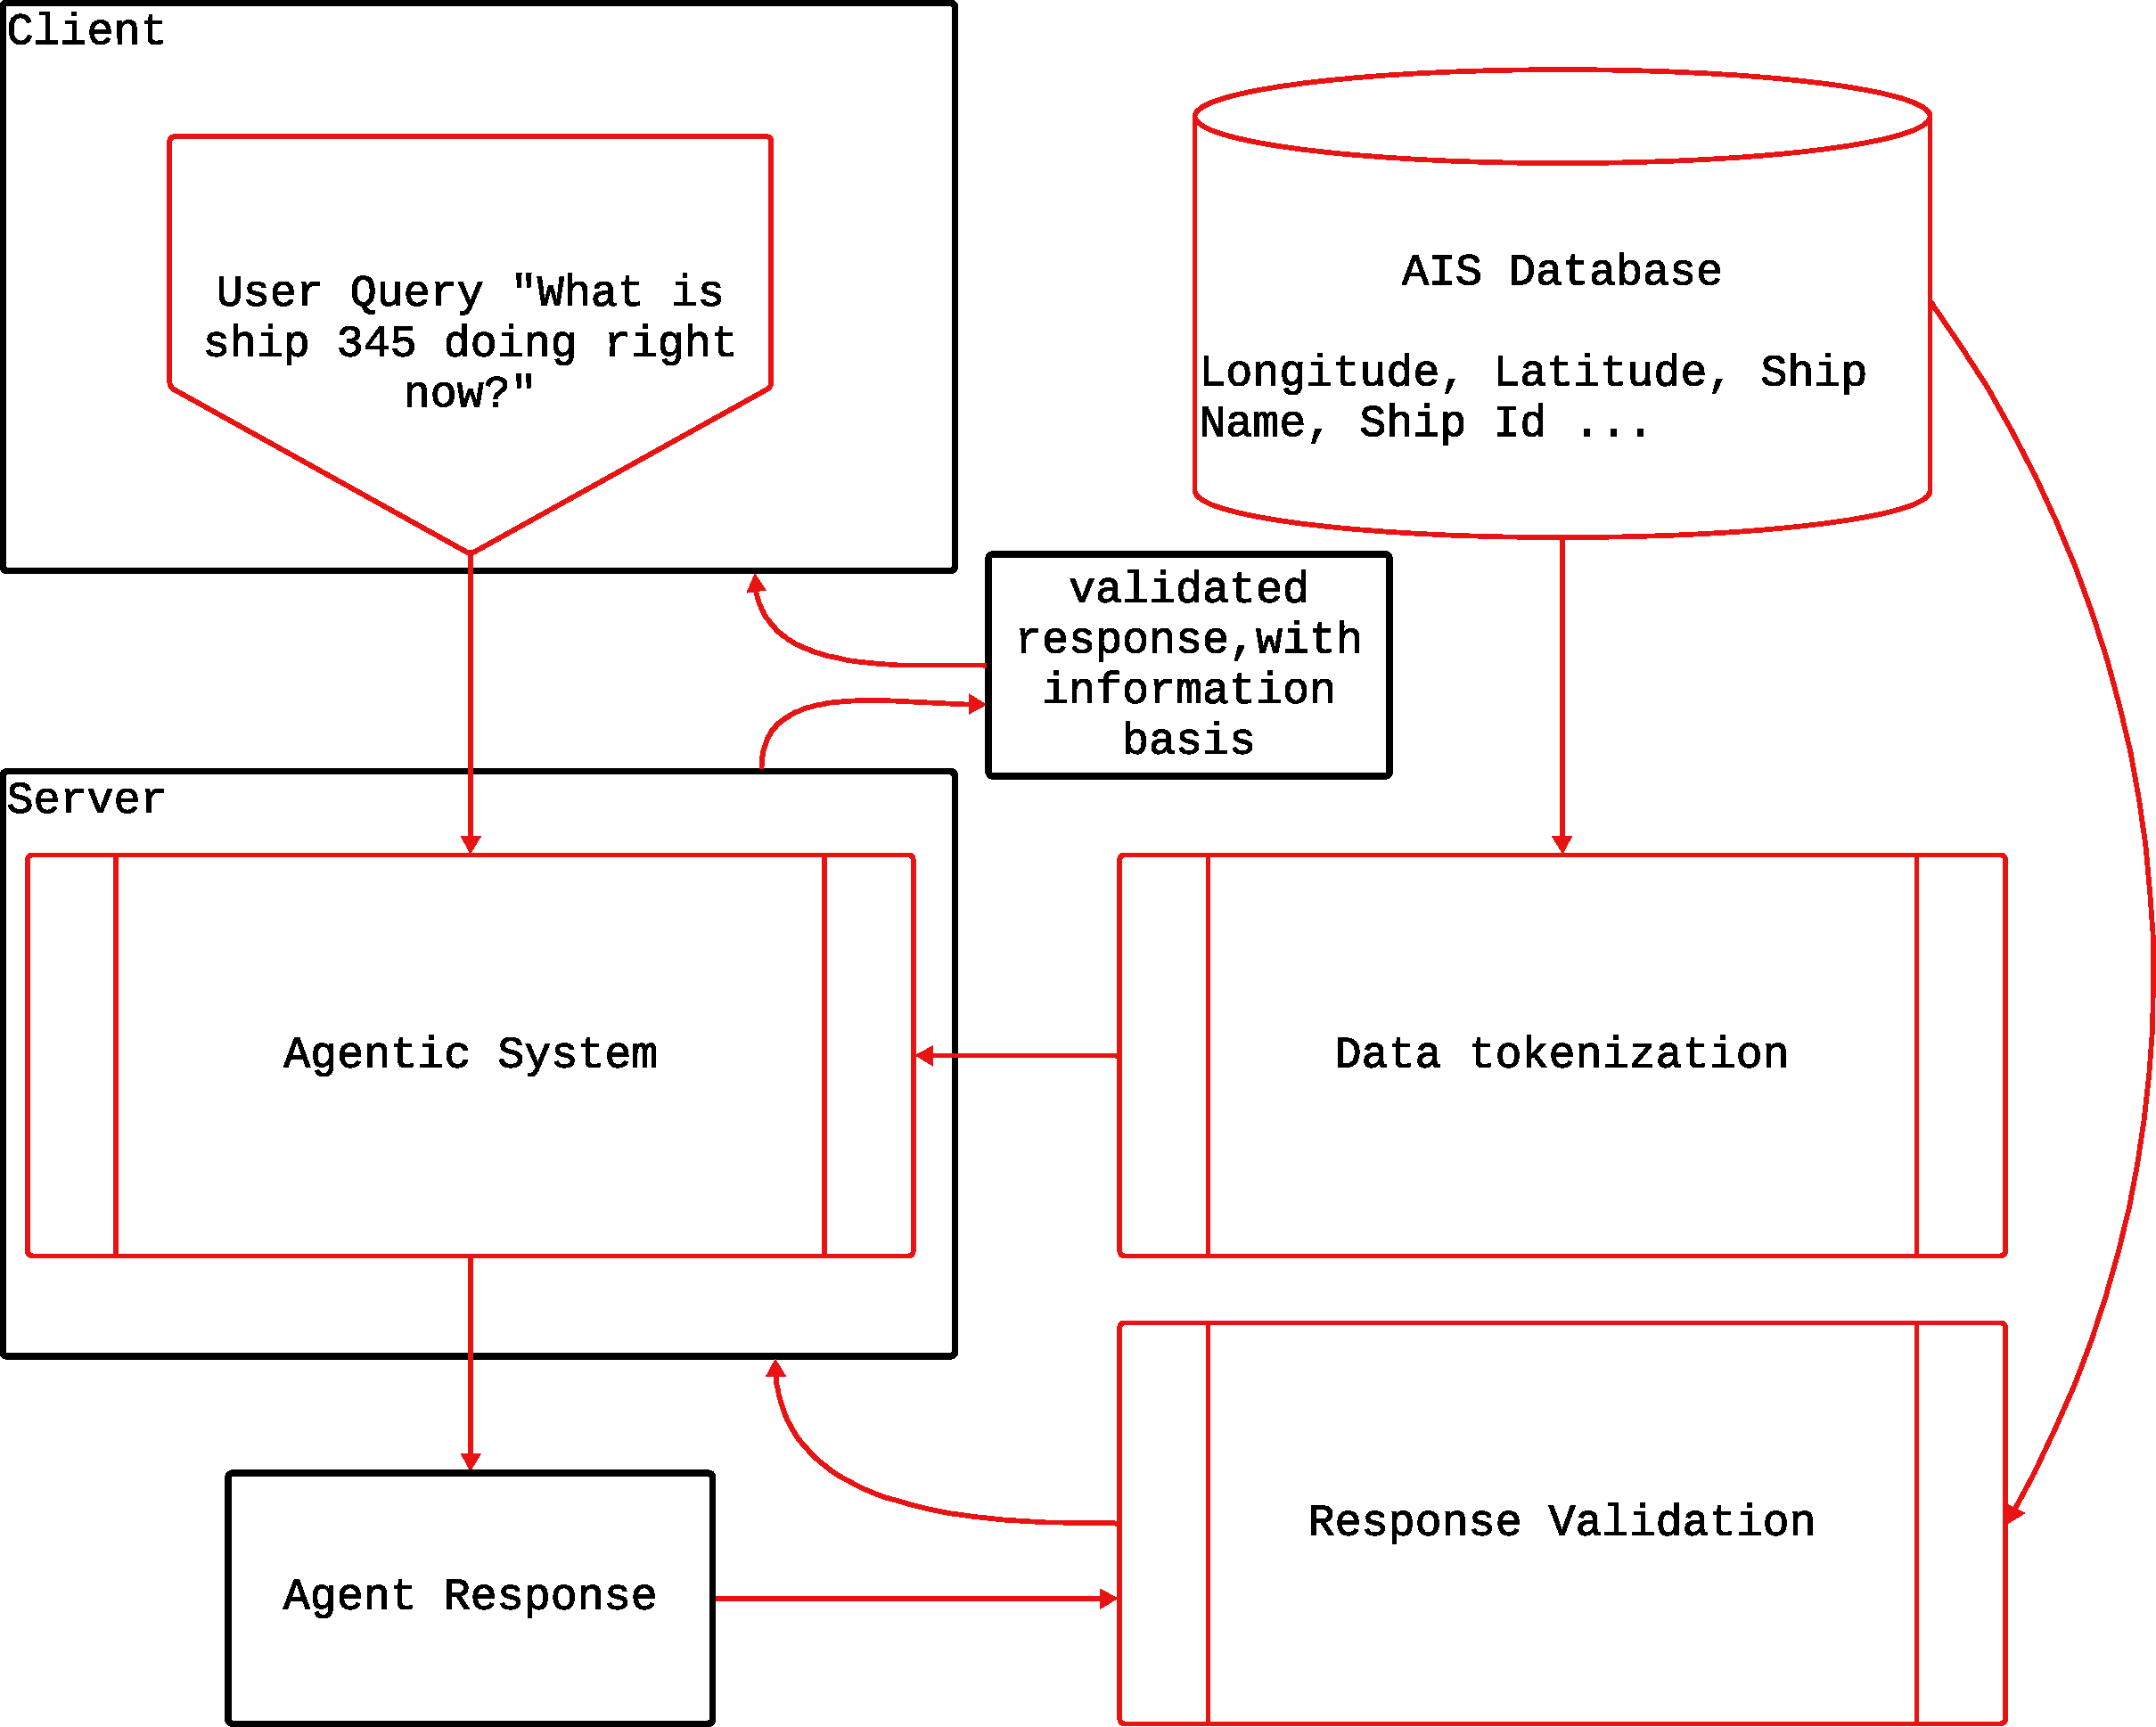
\includegraphics[width=0.5\linewidth]{figs/actintsystem.pdf}
    \caption{Caption}
    \label{fig:placeholder}
\end{figure}

\caption{ACTINT architecture for AIS ingestion, persistent tracking, and LLM-based query answering with evidence and policies.}
\end{figure}

\subsection*{Stage Explanations}
\paragraph{Input.}
The system accepts (i) AIS tabular messages from a feed and (ii) user natural-language questions via an API or UI.
\paragraph{Preprocessing.}
AIS messages are parsed and validated, timestamps are normalized, duplicates removed, and outliers flagged (e.g., impossible speed/position jumps).
\paragraph{Representation (tokens / embeddings / features).}
AIS data is transformed into numerical state/features for tracking plus compact textual/JSON summaries for LLM context.
\paragraph{Model inference.}
The LLM performs tool-augmented reasoning over retrieved vessel data to answer the question and generate a short explanation grounded in evidence.
\paragraph{Postprocessing.}
The output is formatted, checked for evidence compliance, and enriched with key facts (e.g., last known location, heading).
\paragraph{Constraints / policies.}
The system enforces evidence requirements, timeouts, and guardrails against fabricated identifiers/fields.
\paragraph{Output.}
The final answer returns as natural language with traceable support.

% --- (rest of your document can remain unchanged) ---

\section{Initial Model Selection}
The project will begin with open-source LLMs suitable for local or controlled cloud deployment.

\subsection*{Candidate Models}
\begin{itemize}
  \item \textbf{Microsoft Phi family (e.g., Phi-3 Mini/Instruct).} Small, fast models suitable for local inference and rapid iteration.
  \item \textbf{Optional upgrade path:} a stronger open-source instruct model in the 7B--14B range (e.g., Qwen2.5-Instruct, Llama-class instruct models) if reasoning quality is insufficient.
\end{itemize}

\subsection*{Approximate Size}
Phi-class models are typically in the $\sim$3B--4B parameter range. Upgrade candidates range from $\sim$7B to $\sim$14B parameters.

\subsection*{Why this model fits the architecture}
Because ACTINT retrieves the relevant vessel/time window and provides structured context, smaller instruct models can perform well when paired with evidence-focused prompts and validation.

\subsection*{Why not much larger or much smaller?}
Much smaller models may struggle with multi-step reasoning and consistent summaries; much larger models can increase latency/cost and create self-hosting/security complications.

\section{Architectural Constraints}
\subsection*{1) Deployment and Security (Self-Hosted Preference)}
Security requirements may mandate self-hosted inference, pushing the system toward open-source models and controlled data flow.

\subsection*{2) Compute and Memory Limits}
Initial testing resources:
\begin{itemize}
  \item 96 GB VRAM
  \item 64 GB RAM
  \item 32 CPU cores
\end{itemize}

\subsection*{3) Latency and Responsiveness}
The system needs responsive answers; therefore indexed retrieval, bounded windows, caching, and timeouts will be considered in implementation.

\subsection*{4) Data Irregularity and Quality}
AIS updates are irregular and noisy, motivating preprocessing, smoothing, and provenance tracking.

\section{Expected Failure Modes}
\subsection*{Failure Mode 1: Hallucinated or Unsupported Claims}
Type: model failure (and an architectural issue if evidence is not enforced). Mitigation: require citations, validate entities/fields, and optionally constrain outputs to JSON.

\subsection*{Failure Mode 2: Slow Response / Timeouts Under Load}
Type: architectural failure. Mitigation: caching, precomputation, retrieval limits, and multi-model routing.

\subsection*{Explainability Requirement}
ACTINT should present supporting AIS points/derived features and timestamps to justify conclusions.

\section{Semester Roadmap (High Level)}
Weeks 1--2: Architecture design.\\
Weeks 2--4: First prototype development and testing.\\
Weeks 4--6: System validation.\\
Weeks 6--8: Further development based on validation results.\\
Weeks 8--10: Deployment design and implementation.\\
Weeks 10--12: Fine tuning and final adjustments.

\subsection*{Evaluation Metrics}
Early metrics: retrieval correctness, evidence compliance rate, latency (p50/p95), and curated-set task correctness.

\end{document}